\section{Durchschnittliche Verschiebung im nationalen Vergleich}
\subsection{Verteilung der durchschnittlichen Verschiebung unter den Landkreise}
In den folgenden sind die deutschen Landkreise entsprechend dem Durchschnitt der Werte ihrer Zeile in den obigen Matrizen eingefärbt.

In \autoref{fig:average_shift_counties.png} sind die Landkreise entsprechend der Durchschnitte ihrer Zeilen in der rechten unteren Matrix aus \autoref{fig:matrizes_pop_density_counties} bzw. \autoref{fig:matrizes_north_to_south_counties} eingefärbt. Links daneben ist die Verteilung dargestellt.

\begin{figure}[H]
    \centering
    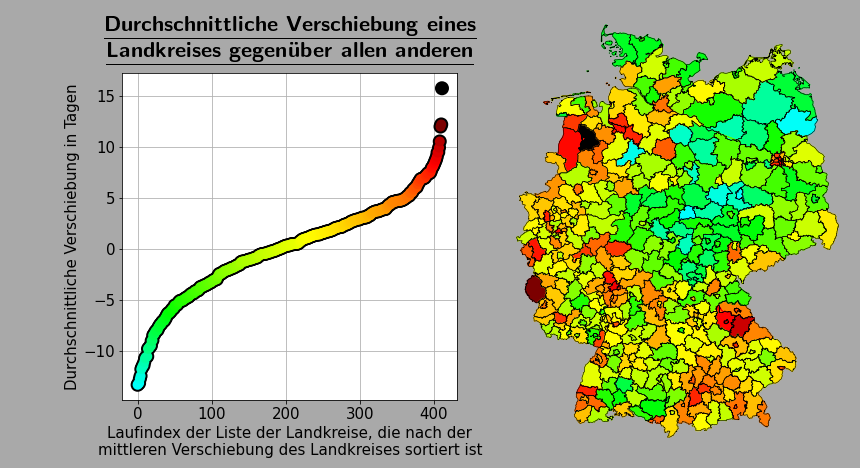
\includegraphics[width = 0.95\textwidth]{figures/Ergebnisse/average_shift_counties.png}
    \caption{Auf der rechten Seite die deutschen Landkreise eingefärbt im Durchschnitt der Maximalwerte der Korrelationen mit allen Landkreisen und Verschiebungen $\tau\in[-50,50]$. Auf der linken Seite die Verteilung dieser Werte.}
    \label{fig:average_shift_counties.png}
\end{figure}

In \autoref{fig:positive_or_negative_shift_counties} sind die Landkreise entsprechend der Durchschnitte ihrer Zeilen in der linken unteren Matrix aus \autoref{fig:matrizes_pop_density_counties} bzw. \autoref{fig:matrizes_north_to_south_counties} eingefärbt. Links daneben ist die Verteilung dargestellt.

\begin{figure}[H]
    \centering
    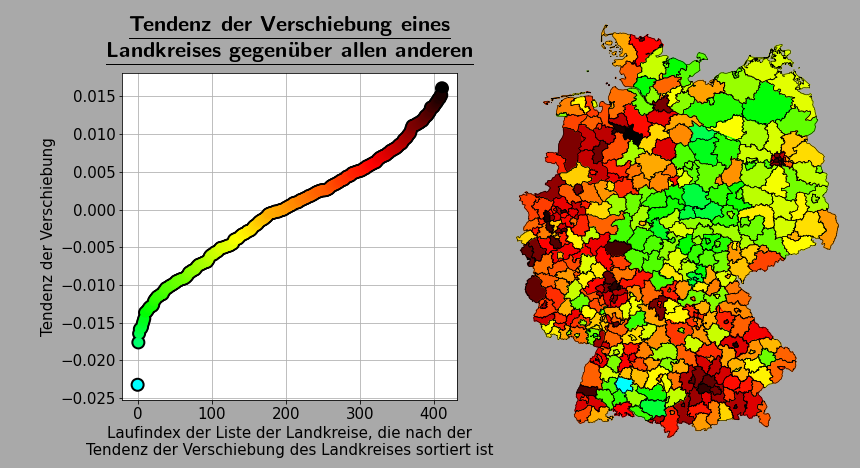
\includegraphics[width = 0.95\textwidth]{figures/Ergebnisse/positive_or_negative_shift_counties.png}
    \caption{Auf der rechten Seite die deutschen Landkreise eingefärbt im Durchschnitt der Differenz der Korrelationswahrscheinlichkeiten der positiven Verschiebungen zu den Korrelationswahrscheinlichkeiten der negativen Verschiebungen der Korrelationen dieses Landkreises mit allen Landkreisen und Verschiebungen $\tau\in[-50,50]$. Auf der linken Seite die Verteilung dieser Werte.}
    \label{fig:positive_or_negative_shift_counties}
\end{figure}



\subsection{Verteilung der durchschnittlichen Verschiebung unter den Regierungsbezirken}
In den folgenden sind die deutschen Regierungsbezirke entsprechend dem Durchschnitt der Werte ihrer Zeile in den obigen Matrizen eingefärbt.

In \autoref{fig:average_shift_districts.png} sind die Regierungsbezirke entsprechend der Durchschnitte ihrer Zeilen in der rechten unteren Matrix aus \autoref{fig:matrizes_pop_density_districts} bzw. \autoref{fig:matrizes_north_to_south_districts} eingefärbt. Links daneben ist die Verteilung dargestellt.

\begin{figure}[H]
    \centering
    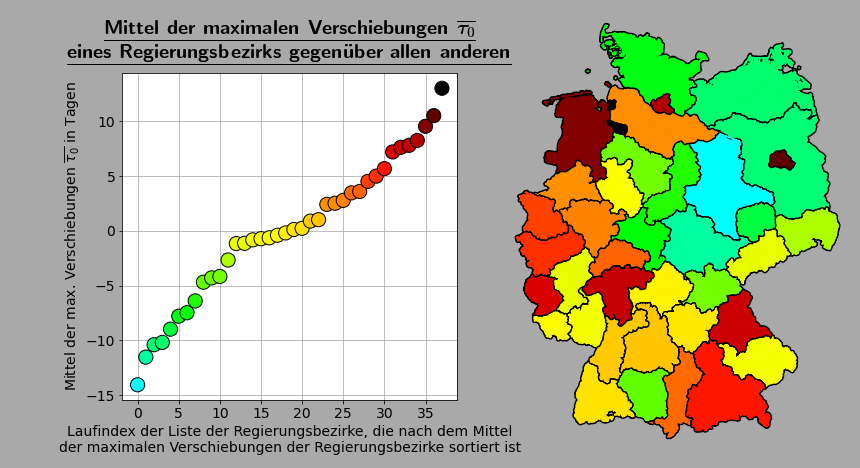
\includegraphics[width = 0.95\textwidth]{figures/Ergebnisse/average_shift_districts.png}
    \caption{Auf der rechten Seite die deutschen Regierungsbezirke eingefärbt im Durchschnitt der Maximalwerte der Korrelationen mit allen Regierungsbezirken und Verschiebungen $\tau\in[-50,50]$. Auf der linken Seite die Verteilung dieser Werte.}
    \label{fig:average_shift_districts.png}
\end{figure}

In \autoref{fig:positive_or_negative_shift_districts} sind die Regierungsbezirke entsprechend der Durchschnitte ihrer Zeilen in der linken unteren Matrix aus \autoref{fig:matrizes_pop_density_districts} bzw. \autoref{fig:matrizes_north_to_south_districts} eingefärbt. Links daneben ist die Verteilung dargestellt.

\begin{figure}[H]
    \centering
    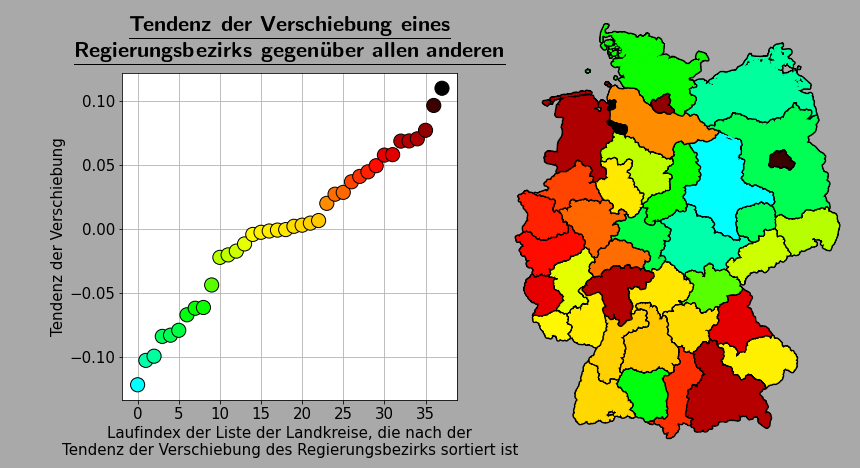
\includegraphics[width = 0.95\textwidth]{figures/Ergebnisse/positive_or_negative_shift_districts.png}
    \caption{Auf der rechten Seite die deutschen Regierungsbezirke eingefärbt im Durchschnitt der Differenz der Korrelationswahrscheinlichkeiten der positiven Verschiebungen zu den Korrelationswahrscheinlichkeiten der negativen Verschiebungen der Korrelationen dieses Regierungsbezirks mit allen Regierungsbezirken und Verschiebungen $\tau\in[-50,50]$. Auf der linken Seite die Verteilung dieser Werte.}
    \label{fig:positive_or_negative_shift_districts}
\end{figure}

